\documentclass[1p]{elsarticle_modified}
%\bibliographystyle{elsarticle-num}

%\usepackage[colorlinks]{hyperref}
%\usepackage{abbrmath_seonhwa} %\Abb, \Ascr, \Acal ,\Abf, \Afrak
\usepackage{amsfonts}
\usepackage{amssymb}
\usepackage{amsmath}
\usepackage{amsthm}
\usepackage{scalefnt}
\usepackage{amsbsy}
\usepackage{kotex}
\usepackage{caption}
\usepackage{subfig}
\usepackage{color}
\usepackage{graphicx}
\usepackage{xcolor} %% white, black, red, green, blue, cyan, magenta, yellow
\usepackage{float}
\usepackage{setspace}
\usepackage{hyperref}

\usepackage{tikz}
\usetikzlibrary{arrows}

\usepackage{multirow}
\usepackage{array} % fixed length table
\usepackage{hhline}

%%%%%%%%%%%%%%%%%%%%%
\makeatletter
\renewcommand*\env@matrix[1][\arraystretch]{%
	\edef\arraystretch{#1}%
	\hskip -\arraycolsep
	\let\@ifnextchar\new@ifnextchar
	\array{*\c@MaxMatrixCols c}}
\makeatother %https://tex.stackexchange.com/questions/14071/how-can-i-increase-the-line-spacing-in-a-matrix
%%%%%%%%%%%%%%%

\usepackage[normalem]{ulem}

\newcommand{\msout}[1]{\ifmmode\text{\sout{\ensuremath{#1}}}\else\sout{#1}\fi}
%SOURCE: \msout is \stkout macro in https://tex.stackexchange.com/questions/20609/strikeout-in-math-mode

\newcommand{\cancel}[1]{
	\ifmmode
	{\color{red}\msout{#1}}
	\else
	{\color{red}\sout{#1}}
	\fi
}

\newcommand{\add}[1]{
	{\color{blue}\uwave{#1}}
}

\newcommand{\replace}[2]{
	\ifmmode
	{\color{red}\msout{#1}}{\color{blue}\uwave{#2}}
	\else
	{\color{red}\sout{#1}}{\color{blue}\uwave{#2}}
	\fi
}

\newcommand{\Sol}{\mathcal{S}} %segment
\newcommand{\D}{D} %diagram
\newcommand{\A}{\mathcal{A}} %arc


%%%%%%%%%%%%%%%%%%%%%%%%%%%%%5 test

\def\sl{\operatorname{\textup{SL}}(2,\Cbb)}
\def\psl{\operatorname{\textup{PSL}}(2,\Cbb)}
\def\quan{\mkern 1mu \triangleright \mkern 1mu}

\theoremstyle{definition}
\newtheorem{thm}{Theorem}[section]
\newtheorem{prop}[thm]{Proposition}
\newtheorem{lem}[thm]{Lemma}
\newtheorem{ques}[thm]{Question}
\newtheorem{cor}[thm]{Corollary}
\newtheorem{defn}[thm]{Definition}
\newtheorem{exam}[thm]{Example}
\newtheorem{rmk}[thm]{Remark}
\newtheorem{alg}[thm]{Algorithm}

\newcommand{\I}{\sqrt{-1}}
\begin{document}

%\begin{frontmatter}
%
%\title{Boundary parabolic representations of knots up to 8 crossings}
%
%%% Group authors per affiliation:
%\author{Yunhi Cho} 
%\address{Department of Mathematics, University of Seoul, Seoul, Korea}
%\ead{yhcho@uos.ac.kr}
%
%
%\author{Seonhwa Kim} %\fnref{s_kim}}
%\address{Center for Geometry and Physics, Institute for Basic Science, Pohang, 37673, Korea}
%\ead{ryeona17@ibs.re.kr}
%
%\author{Hyuk Kim}
%\address{Department of Mathematical Sciences, Seoul National University, Seoul 08826, Korea}
%\ead{hyukkim@snu.ac.kr}
%
%\author{Seokbeom Yoon}
%\address{Department of Mathematical Sciences, Seoul National University, Seoul, 08826,  Korea}
%\ead{sbyoon15@snu.ac.kr}
%
%\begin{abstract}
%We find all boundary parabolic representation of knots up to 8 crossings.
%
%\end{abstract}
%\begin{keyword}
%    \MSC[2010] 57M25 
%\end{keyword}
%
%\end{frontmatter}

%\linenumbers
%\tableofcontents
%
\newcommand\colored[1]{\textcolor{white}{\rule[-0.35ex]{0.8em}{1.4ex}}\kern-0.8em\color{red} #1}%
%\newcommand\colored[1]{\textcolor{white}{ #1}\kern-2.17ex	\textcolor{white}{ #1}\kern-1.81ex	\textcolor{white}{ #1}\kern-2.15ex\color{red}#1	}

{\Large $\underline{12a_{0859}~(K12a_{0859})}$}

\setlength{\tabcolsep}{10pt}
\renewcommand{\arraystretch}{1.6}
\vspace{1cm}\begin{tabular}{m{100pt}>{\centering\arraybackslash}m{274pt}}
\multirow{5}{120pt}{
	\centering
	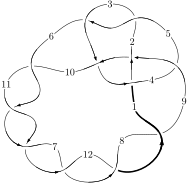
\includegraphics[width=112pt]{../../../GIT/diagram.site/Diagrams/png/1660_12a_0859.png}\\
\ \ \ A knot diagram\footnotemark}&
\allowdisplaybreaks
\textbf{Linearized knot diagam} \\
\cline{2-2}
 &
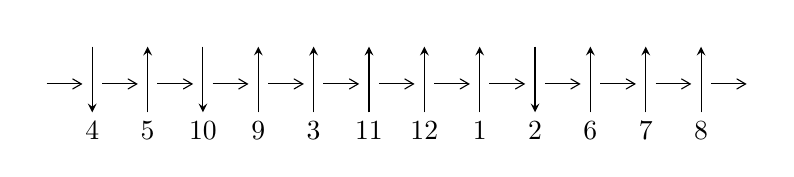
\begin{tikzpicture}[x=20pt, y=17pt]
	% nodes
	\node (C0) at (0, 0) {};
	\node (C1) at (1, 0) {};
	\node (C1U) at (1, +1) {};
	\node (C1D) at (1, -1) {4};

	\node (C2) at (2, 0) {};
	\node (C2U) at (2, +1) {};
	\node (C2D) at (2, -1) {5};

	\node (C3) at (3, 0) {};
	\node (C3U) at (3, +1) {};
	\node (C3D) at (3, -1) {10};

	\node (C4) at (4, 0) {};
	\node (C4U) at (4, +1) {};
	\node (C4D) at (4, -1) {9};

	\node (C5) at (5, 0) {};
	\node (C5U) at (5, +1) {};
	\node (C5D) at (5, -1) {3};

	\node (C6) at (6, 0) {};
	\node (C6U) at (6, +1) {};
	\node (C6D) at (6, -1) {11};

	\node (C7) at (7, 0) {};
	\node (C7U) at (7, +1) {};
	\node (C7D) at (7, -1) {12};

	\node (C8) at (8, 0) {};
	\node (C8U) at (8, +1) {};
	\node (C8D) at (8, -1) {1};

	\node (C9) at (9, 0) {};
	\node (C9U) at (9, +1) {};
	\node (C9D) at (9, -1) {2};

	\node (C10) at (10, 0) {};
	\node (C10U) at (10, +1) {};
	\node (C10D) at (10, -1) {6};

	\node (C11) at (11, 0) {};
	\node (C11U) at (11, +1) {};
	\node (C11D) at (11, -1) {7};

	\node (C12) at (12, 0) {};
	\node (C12U) at (12, +1) {};
	\node (C12D) at (12, -1) {8};
	\node (C13) at (13, 0) {};

	% arrows
	\draw[->,>={angle 60}]
	(C0) edge (C1) (C1) edge (C2) (C2) edge (C3) (C3) edge (C4) (C4) edge (C5) (C5) edge (C6) (C6) edge (C7) (C7) edge (C8) (C8) edge (C9) (C9) edge (C10) (C10) edge (C11) (C11) edge (C12) (C12) edge (C13) ;	\draw[->,>=stealth]
	(C1U) edge (C1D) (C2D) edge (C2U) (C3U) edge (C3D) (C4D) edge (C4U) (C5D) edge (C5U) (C6D) edge (C6U) (C7D) edge (C7U) (C8D) edge (C8U) (C9U) edge (C9D) (C10D) edge (C10U) (C11D) edge (C11U) (C12D) edge (C12U) ;
	\end{tikzpicture} \\
\hhline{~~} \\& 
\textbf{Solving Sequence} \\ \cline{2-2} 
 &
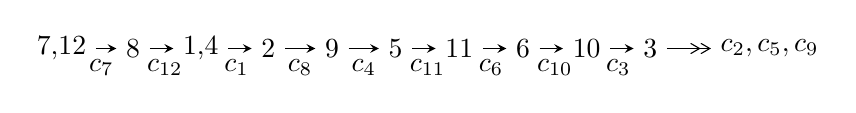
\begin{tikzpicture}[x=23pt, y=7pt]
	% node
	\node (A0) at (-1/8, 0) {7,12};
	\node (A1) at (1, 0) {8};
	\node (A2) at (33/16, 0) {1,4};
	\node (A3) at (25/8, 0) {2};
	\node (A4) at (33/8, 0) {9};
	\node (A5) at (41/8, 0) {5};
	\node (A6) at (49/8, 0) {11};
	\node (A7) at (57/8, 0) {6};
	\node (A8) at (65/8, 0) {10};
	\node (A9) at (73/8, 0) {3};
	\node (C1) at (1/2, -1) {$c_{7}$};
	\node (C2) at (3/2, -1) {$c_{12}$};
	\node (C3) at (21/8, -1) {$c_{1}$};
	\node (C4) at (29/8, -1) {$c_{8}$};
	\node (C5) at (37/8, -1) {$c_{4}$};
	\node (C6) at (45/8, -1) {$c_{11}$};
	\node (C7) at (53/8, -1) {$c_{6}$};
	\node (C8) at (61/8, -1) {$c_{10}$};
	\node (C9) at (69/8, -1) {$c_{3}$};
	\node (A10) at (11, 0) {$c_{2},c_{5},c_{9}$};

	% edge
	\draw[->,>=stealth]	
	(A0) edge (A1) (A1) edge (A2) (A2) edge (A3) (A3) edge (A4) (A4) edge (A5) (A5) edge (A6) (A6) edge (A7) (A7) edge (A8) (A8) edge (A9) ;
	\draw[->>,>={angle 60}]	
	(A9) edge (A10);
\end{tikzpicture} \\ 

\end{tabular} \\

\footnotetext{
The image of knot diagram is generated by the software ``\textbf{Draw programme}" developed by Andrew Bartholomew(\url{http://www.layer8.co.uk/maths/draw/index.htm\#Running-draw}), where we modified some parts for our purpose(\url{https://github.com/CATsTAILs/LinksPainter}).
}\phantom \\ \newline 
\centering \textbf{Ideals for irreducible components\footnotemark of $X_{\text{par}}$} 
 
\begin{align*}
I^u_{1}&=\langle 
-6396631669231 u^{40}+14505431853193 u^{39}+\cdots+4256439997929 b-11189757056882,\\
\phantom{I^u_{1}}&\phantom{= \langle  }-1233760383109 u^{40}+3011254162855 u^{39}+\cdots+608062856847 a-1195143358109,\\
\phantom{I^u_{1}}&\phantom{= \langle  }u^{41}-2 u^{40}+\cdots+5 u+1\rangle \\
I^u_{2}&=\langle 
b+1,\;a- u+1,\;u^2- u-1\rangle \\
\\
\end{align*}
\raggedright * 2 irreducible components of $\dim_{\mathbb{C}}=0$, with total 43 representations.\\
\footnotetext{All coefficients of polynomials are rational numbers. But the coefficients are sometimes approximated in decimal forms when there is not enough margin.}
\newpage
\renewcommand{\arraystretch}{1}
\centering \section*{I. $I^u_{1}= \langle -6.40\times10^{12} u^{40}+1.45\times10^{13} u^{39}+\cdots+4.26\times10^{12} b-1.12\times10^{13},\;-1.23\times10^{12} u^{40}+3.01\times10^{12} u^{39}+\cdots+6.08\times10^{11} a-1.20\times10^{12},\;u^{41}-2 u^{40}+\cdots+5 u+1 \rangle$}
\flushleft \textbf{(i) Arc colorings}\\
\begin{tabular}{m{7pt} m{180pt} m{7pt} m{180pt} }
\flushright $a_{7}=$&$\begin{pmatrix}1\\0\end{pmatrix}$ \\
\flushright $a_{12}=$&$\begin{pmatrix}0\\u\end{pmatrix}$ \\
\flushright $a_{8}=$&$\begin{pmatrix}1\\- u^2\end{pmatrix}$ \\
\flushright $a_{1}=$&$\begin{pmatrix}u\\- u^3+u\end{pmatrix}$ \\
\flushright $a_{4}=$&$\begin{pmatrix}2.02900 u^{40}-4.95221 u^{39}+\cdots+15.4220 u+1.96549\\1.50281 u^{40}-3.40788 u^{39}+\cdots+11.3789 u+2.62890\end{pmatrix}$ \\
\flushright $a_{2}=$&$\begin{pmatrix}0.644891 u^{40}-0.202904 u^{39}+\cdots-3.45077 u+0.277543\\-1.08688 u^{40}-0.397073 u^{39}+\cdots+2.94691 u+0.644891\end{pmatrix}$ \\
\flushright $a_{9}=$&$\begin{pmatrix}- u^2+1\\u^4-2 u^2\end{pmatrix}$ \\
\flushright $a_{5}=$&$\begin{pmatrix}3.70468 u^{40}-8.56110 u^{39}+\cdots+27.1650 u+4.70761\\-0.0447870 u^{40}-1.39889 u^{39}+\cdots+9.37521 u+1.50458\end{pmatrix}$ \\
\flushright $a_{11}=$&$\begin{pmatrix}- u\\u\end{pmatrix}$ \\
\flushright $a_{6}=$&$\begin{pmatrix}- u^2+1\\u^2\end{pmatrix}$ \\
\flushright $a_{10}=$&$\begin{pmatrix}u^3-2 u\\- u^3+u\end{pmatrix}$ \\
\flushright $a_{3}=$&$\begin{pmatrix}3.76543 u^{40}-8.75980 u^{39}+\cdots+26.5272 u+5.57736\\0.0237411 u^{40}-1.60020 u^{39}+\cdots+9.41064 u+1.56557\end{pmatrix}$\\&\end{tabular}
\flushleft \textbf{(ii) Obstruction class $= -1$}\\~\\
\flushleft \textbf{(iii) Cusp Shapes $= -\frac{47359814646430}{1418813332643} u^{40}+\frac{116172431816127}{1418813332643} u^{39}+\cdots-\frac{243964640346834}{1418813332643} u-\frac{78234342263103}{1418813332643}$}\\~\\
\newpage\renewcommand{\arraystretch}{1}
\flushleft \textbf{(iv) u-Polynomials at the component}\newline \\
\begin{tabular}{m{50pt}|m{274pt}}
Crossings & \hspace{64pt}u-Polynomials at each crossing \\
\hline $$\begin{aligned}c_{1}\end{aligned}$$&$\begin{aligned}
&u^{41}-7 u^{40}+\cdots+20 u+4
\end{aligned}$\\
\hline $$\begin{aligned}c_{2},c_{5}\end{aligned}$$&$\begin{aligned}
&u^{41}+3 u^{40}+\cdots+14 u-1
\end{aligned}$\\
\hline $$\begin{aligned}c_{3}\end{aligned}$$&$\begin{aligned}
&u^{41}+2 u^{40}+\cdots-7931 u+3953
\end{aligned}$\\
\hline $$\begin{aligned}c_{4}\end{aligned}$$&$\begin{aligned}
&u^{41}+4 u^{40}+\cdots+197 u-19
\end{aligned}$\\
\hline $$\begin{aligned}c_{6},c_{7},c_{8}\\c_{10},c_{11},c_{12}\end{aligned}$$&$\begin{aligned}
&u^{41}+2 u^{40}+\cdots+5 u-1
\end{aligned}$\\
\hline $$\begin{aligned}c_{9}\end{aligned}$$&$\begin{aligned}
&u^{41}-2 u^{40}+\cdots- u+1
\end{aligned}$\\
\hline
\end{tabular}\\~\\
\newpage\renewcommand{\arraystretch}{1}
\flushleft \textbf{(v) Riley Polynomials at the component}\newline \\
\begin{tabular}{m{50pt}|m{274pt}}
Crossings & \hspace{64pt}Riley Polynomials at each crossing \\
\hline $$\begin{aligned}c_{1}\end{aligned}$$&$\begin{aligned}
&y^{41}+15 y^{40}+\cdots+104 y-16
\end{aligned}$\\
\hline $$\begin{aligned}c_{2},c_{5}\end{aligned}$$&$\begin{aligned}
&y^{41}-35 y^{40}+\cdots+102 y-1
\end{aligned}$\\
\hline $$\begin{aligned}c_{3}\end{aligned}$$&$\begin{aligned}
&y^{41}-12 y^{40}+\cdots-126297725 y-15626209
\end{aligned}$\\
\hline $$\begin{aligned}c_{4}\end{aligned}$$&$\begin{aligned}
&y^{41}-56 y^{40}+\cdots+33831 y-361
\end{aligned}$\\
\hline $$\begin{aligned}c_{6},c_{7},c_{8}\\c_{10},c_{11},c_{12}\end{aligned}$$&$\begin{aligned}
&y^{41}-60 y^{40}+\cdots+3 y-1
\end{aligned}$\\
\hline $$\begin{aligned}c_{9}\end{aligned}$$&$\begin{aligned}
&y^{41}+4 y^{40}+\cdots+3 y-1
\end{aligned}$\\
\hline
\end{tabular}\\~\\
\newpage\flushleft \textbf{(vi) Complex Volumes and Cusp Shapes}
$$\begin{array}{c|c|c}  
\text{Solutions to }I^u_{1}& \I (\text{vol} + \sqrt{-1}CS) & \text{Cusp shape}\\
 \hline 
\begin{aligned}
u &= -0.650909 + 0.546359 I \\
a &= -0.342020 + 0.264851 I \\
b &= \phantom{-}0.419018 - 0.668068 I\end{aligned}
 & \phantom{-}5.06652 + 0.73720 I & \phantom{-}15.9081 - 0.1824 I \\ \hline\begin{aligned}
u &= -0.650909 - 0.546359 I \\
a &= -0.342020 - 0.264851 I \\
b &= \phantom{-}0.419018 + 0.668068 I\end{aligned}
 & \phantom{-}5.06652 - 0.73720 I & \phantom{-}15.9081 + 0.1824 I \\ \hline\begin{aligned}
u &= \phantom{-}0.698668 + 0.479441 I \\
a &= \phantom{-}0.153099 - 0.435306 I \\
b &= -0.188432 + 1.146320 I\end{aligned}
 & \phantom{-}5.52631 + 8.23953 I & \phantom{-}13.0991 - 8.0874 I \\ \hline\begin{aligned}
u &= \phantom{-}0.698668 - 0.479441 I \\
a &= \phantom{-}0.153099 + 0.435306 I \\
b &= -0.188432 - 1.146320 I\end{aligned}
 & \phantom{-}5.52631 - 8.23953 I & \phantom{-}13.0991 + 8.0874 I \\ \hline\begin{aligned}
u &= -0.814283\phantom{ +0.000000I} \\
a &= \phantom{-}0.0171192\phantom{ +0.000000I} \\
b &= -0.681057\phantom{ +0.000000I}\end{aligned}
 & \phantom{-}1.28070\phantom{ +0.000000I} & \phantom{-}6.70620\phantom{ +0.000000I} \\ \hline\begin{aligned}
u &= \phantom{-}1.247790 + 0.069918 I \\
a &= \phantom{-}0.862844 + 1.105030 I \\
b &= -0.437368 - 0.248810 I\end{aligned}
 & \phantom{-}6.66501 + 1.00107 I & \phantom{-0.000000 } 0 \\ \hline\begin{aligned}
u &= \phantom{-}1.247790 - 0.069918 I \\
a &= \phantom{-}0.862844 - 1.105030 I \\
b &= -0.437368 + 0.248810 I\end{aligned}
 & \phantom{-}6.66501 - 1.00107 I & \phantom{-0.000000 } 0 \\ \hline\begin{aligned}
u &= \phantom{-}1.28100\phantom{ +0.000000I} \\
a &= -3.02459\phantom{ +0.000000I} \\
b &= \phantom{-}2.36170\phantom{ +0.000000I}\end{aligned}
 & \phantom{-}8.47175\phantom{ +0.000000I} & \phantom{-0.000000 } 0 \\ \hline\begin{aligned}
u &= -1.290140 + 0.118342 I \\
a &= \phantom{-}0.175331 - 1.312220 I \\
b &= -0.325850 - 0.263604 I\end{aligned}
 & \phantom{-}6.85332 - 5.09177 I & \phantom{-0.000000 } 0 \\ \hline\begin{aligned}
u &= -1.290140 - 0.118342 I \\
a &= \phantom{-}0.175331 + 1.312220 I \\
b &= -0.325850 + 0.263604 I\end{aligned}
 & \phantom{-}6.85332 + 5.09177 I & \phantom{-0.000000 } 0\\
 \hline 
 \end{array}$$\newpage$$\begin{array}{c|c|c}  
\text{Solutions to }I^u_{1}& \I (\text{vol} + \sqrt{-1}CS) & \text{Cusp shape}\\
 \hline 
\begin{aligned}
u &= -1.328540 + 0.037966 I \\
a &= \phantom{-}0.004954 - 0.826516 I \\
b &= \phantom{-}1.188080 - 0.254233 I\end{aligned}
 & \phantom{-}10.93780 - 2.08245 I & \phantom{-0.000000 } 0 \\ \hline\begin{aligned}
u &= -1.328540 - 0.037966 I \\
a &= \phantom{-}0.004954 + 0.826516 I \\
b &= \phantom{-}1.188080 + 0.254233 I\end{aligned}
 & \phantom{-}10.93780 + 2.08245 I & \phantom{-0.000000 } 0 \\ \hline\begin{aligned}
u &= \phantom{-}0.659491 + 0.101039 I \\
a &= \phantom{-}1.78864 + 0.62056 I \\
b &= -0.599129 - 0.924522 I\end{aligned}
 & \phantom{-}4.32500 + 1.61112 I & \phantom{-}18.8008 - 4.7797 I \\ \hline\begin{aligned}
u &= \phantom{-}0.659491 - 0.101039 I \\
a &= \phantom{-}1.78864 - 0.62056 I \\
b &= -0.599129 + 0.924522 I\end{aligned}
 & \phantom{-}4.32500 - 1.61112 I & \phantom{-}18.8008 + 4.7797 I \\ \hline\begin{aligned}
u &= \phantom{-}0.576581 + 0.288116 I \\
a &= -0.354068 + 1.004510 I \\
b &= \phantom{-}0.372702 - 1.123810 I\end{aligned}
 & \phantom{-}0.71083 + 3.70513 I & \phantom{-}10.09368 - 9.17012 I \\ \hline\begin{aligned}
u &= \phantom{-}0.576581 - 0.288116 I \\
a &= -0.354068 - 1.004510 I \\
b &= \phantom{-}0.372702 + 1.123810 I\end{aligned}
 & \phantom{-}0.71083 - 3.70513 I & \phantom{-}10.09368 + 9.17012 I \\ \hline\begin{aligned}
u &= -0.043590 + 0.639393 I \\
a &= \phantom{-}1.046310 - 0.645722 I \\
b &= \phantom{-}0.0798501 + 0.0811079 I\end{aligned}
 & \phantom{-}3.26424 - 4.59923 I & \phantom{-}10.62501 + 5.19359 I \\ \hline\begin{aligned}
u &= -0.043590 - 0.639393 I \\
a &= \phantom{-}1.046310 + 0.645722 I \\
b &= \phantom{-}0.0798501 - 0.0811079 I\end{aligned}
 & \phantom{-}3.26424 + 4.59923 I & \phantom{-}10.62501 - 5.19359 I \\ \hline\begin{aligned}
u &= -1.344360 + 0.232182 I \\
a &= -0.353369 + 1.278910 I \\
b &= -0.006247 - 0.161367 I\end{aligned}
 & \phantom{-}12.2007 - 10.7908 I & \phantom{-0.000000 } 0 \\ \hline\begin{aligned}
u &= -1.344360 - 0.232182 I \\
a &= -0.353369 - 1.278910 I \\
b &= -0.006247 + 0.161367 I\end{aligned}
 & \phantom{-}12.2007 + 10.7908 I & \phantom{-0.000000 } 0\\
 \hline 
 \end{array}$$\newpage$$\begin{array}{c|c|c}  
\text{Solutions to }I^u_{1}& \I (\text{vol} + \sqrt{-1}CS) & \text{Cusp shape}\\
 \hline 
\begin{aligned}
u &= \phantom{-}1.348660 + 0.276814 I \\
a &= -0.414645 - 0.555057 I \\
b &= -0.165637 - 0.010708 I\end{aligned}
 & \phantom{-}11.56960 + 2.23576 I & \phantom{-0.000000 } 0 \\ \hline\begin{aligned}
u &= \phantom{-}1.348660 - 0.276814 I \\
a &= -0.414645 + 0.555057 I \\
b &= -0.165637 + 0.010708 I\end{aligned}
 & \phantom{-}11.56960 - 2.23576 I & \phantom{-0.000000 } 0 \\ \hline\begin{aligned}
u &= -0.497845 + 0.153887 I \\
a &= -0.345928 - 0.229979 I \\
b &= -0.477639 + 0.446316 I\end{aligned}
 & \phantom{-}0.963123 - 0.222847 I & \phantom{-}11.33687 + 1.79100 I \\ \hline\begin{aligned}
u &= -0.497845 - 0.153887 I \\
a &= -0.345928 + 0.229979 I \\
b &= -0.477639 - 0.446316 I\end{aligned}
 & \phantom{-}0.963123 + 0.222847 I & \phantom{-}11.33687 - 1.79100 I \\ \hline\begin{aligned}
u &= -0.503963\phantom{ +0.000000I} \\
a &= \phantom{-}4.08982\phantom{ +0.000000I} \\
b &= \phantom{-}2.61045\phantom{ +0.000000I}\end{aligned}
 & \phantom{-}2.49303\phantom{ +0.000000I} & -73.8380\phantom{ +0.000000I} \\ \hline\begin{aligned}
u &= \phantom{-}0.041427 + 0.380391 I \\
a &= -1.47501 + 1.25938 I \\
b &= \phantom{-}0.223887 + 0.085512 I\end{aligned}
 & -0.87754 - 1.43971 I & \phantom{-}1.57134 + 2.80893 I \\ \hline\begin{aligned}
u &= \phantom{-}0.041427 - 0.380391 I \\
a &= -1.47501 - 1.25938 I \\
b &= \phantom{-}0.223887 - 0.085512 I\end{aligned}
 & -0.87754 + 1.43971 I & \phantom{-}1.57134 - 2.80893 I \\ \hline\begin{aligned}
u &= \phantom{-}1.66053\phantom{ +0.000000I} \\
a &= \phantom{-}0.443601\phantom{ +0.000000I} \\
b &= -0.446168\phantom{ +0.000000I}\end{aligned}
 & \phantom{-}10.1068\phantom{ +0.000000I} & \phantom{-0.000000 } 0 \\ \hline\begin{aligned}
u &= -0.150168 + 0.199500 I \\
a &= -3.03352 + 0.19155 I \\
b &= -0.797576 + 0.621794 I\end{aligned}
 & \phantom{-}1.94826 - 0.63992 I & \phantom{-}4.80549 - 1.01730 I \\ \hline\begin{aligned}
u &= -0.150168 - 0.199500 I \\
a &= -3.03352 - 0.19155 I \\
b &= -0.797576 - 0.621794 I\end{aligned}
 & \phantom{-}1.94826 + 0.63992 I & \phantom{-}4.80549 + 1.01730 I\\
 \hline 
 \end{array}$$\newpage$$\begin{array}{c|c|c}  
\text{Solutions to }I^u_{1}& \I (\text{vol} + \sqrt{-1}CS) & \text{Cusp shape}\\
 \hline 
\begin{aligned}
u &= -1.80288 + 0.01775 I \\
a &= -0.75332 + 2.11781 I \\
b &= \phantom{-}1.72917 - 4.38308 I\end{aligned}
 & \phantom{-}17.9481 - 1.4034 I & \phantom{-0.000000 } 0 \\ \hline\begin{aligned}
u &= -1.80288 - 0.01775 I \\
a &= -0.75332 - 2.11781 I \\
b &= \phantom{-}1.72917 + 4.38308 I\end{aligned}
 & \phantom{-}17.9481 + 1.4034 I & \phantom{-0.000000 } 0 \\ \hline\begin{aligned}
u &= -1.81126\phantom{ +0.000000I} \\
a &= \phantom{-}2.44844\phantom{ +0.000000I} \\
b &= -5.97707\phantom{ +0.000000I}\end{aligned}
 & -19.5212\phantom{ +0.000000I} & \phantom{-0.000000 } 0 \\ \hline\begin{aligned}
u &= \phantom{-}1.81283 + 0.02856 I \\
a &= \phantom{-}0.40071 - 2.86621 I \\
b &= -0.63518 + 5.58995 I\end{aligned}
 & \phantom{-}18.3589 + 5.7706 I & \phantom{-0.000000 } 0 \\ \hline\begin{aligned}
u &= \phantom{-}1.81283 - 0.02856 I \\
a &= \phantom{-}0.40071 + 2.86621 I \\
b &= -0.63518 - 5.58995 I\end{aligned}
 & \phantom{-}18.3589 - 5.7706 I & \phantom{-0.000000 } 0 \\ \hline\begin{aligned}
u &= \phantom{-}1.82183 + 0.00897 I \\
a &= -1.28360 - 2.01039 I \\
b &= \phantom{-}1.99257 + 3.92606 I\end{aligned}
 & -16.7931 + 2.3034 I & \phantom{-0.000000 } 0 \\ \hline\begin{aligned}
u &= \phantom{-}1.82183 - 0.00897 I \\
a &= -1.28360 + 2.01039 I \\
b &= \phantom{-}1.99257 - 3.92606 I\end{aligned}
 & -16.7931 - 2.3034 I & \phantom{-0.000000 } 0 \\ \hline\begin{aligned}
u &= \phantom{-}1.82503 + 0.05956 I \\
a &= \phantom{-}0.04404 + 2.55326 I \\
b &= -0.10800 - 5.18854 I\end{aligned}
 & -15.5464 + 12.1966 I & \phantom{-0.000000 } 0 \\ \hline\begin{aligned}
u &= \phantom{-}1.82503 - 0.05956 I \\
a &= \phantom{-}0.04404 - 2.55326 I \\
b &= -0.10800 + 5.18854 I\end{aligned}
 & -15.5464 - 12.1966 I & \phantom{-0.000000 } 0 \\ \hline\begin{aligned}
u &= -1.82989 + 0.06825 I \\
a &= \phantom{-}0.39236 - 1.61771 I \\
b &= -0.69814 + 3.25968 I\end{aligned}
 & -16.1413 - 3.8895 I & \phantom{-0.000000 } 0\\
 \hline 
 \end{array}$$\newpage$$\begin{array}{c|c|c}  
\text{Solutions to }I^u_{1}& \I (\text{vol} + \sqrt{-1}CS) & \text{Cusp shape}\\
 \hline 
\begin{aligned}
u &= -1.82989 - 0.06825 I \\
a &= \phantom{-}0.39236 + 1.61771 I \\
b &= -0.69814 - 3.25968 I\end{aligned}
 & -16.1413 + 3.8895 I & \phantom{-0.000000 } 0\\
 \hline 
 \end{array}$$\newpage\newpage\renewcommand{\arraystretch}{1}
\centering \section*{II. $I^u_{2}= \langle b+1,\;a- u+1,\;u^2- u-1 \rangle$}
\flushleft \textbf{(i) Arc colorings}\\
\begin{tabular}{m{7pt} m{180pt} m{7pt} m{180pt} }
\flushright $a_{7}=$&$\begin{pmatrix}1\\0\end{pmatrix}$ \\
\flushright $a_{12}=$&$\begin{pmatrix}0\\u\end{pmatrix}$ \\
\flushright $a_{8}=$&$\begin{pmatrix}1\\- u-1\end{pmatrix}$ \\
\flushright $a_{1}=$&$\begin{pmatrix}u\\- u-1\end{pmatrix}$ \\
\flushright $a_{4}=$&$\begin{pmatrix}u-1\\-1\end{pmatrix}$ \\
\flushright $a_{2}=$&$\begin{pmatrix}u\\- u-1\end{pmatrix}$ \\
\flushright $a_{9}=$&$\begin{pmatrix}- u\\u\end{pmatrix}$ \\
\flushright $a_{5}=$&$\begin{pmatrix}u-2\\0\end{pmatrix}$ \\
\flushright $a_{11}=$&$\begin{pmatrix}- u\\u\end{pmatrix}$ \\
\flushright $a_{6}=$&$\begin{pmatrix}- u\\u+1\end{pmatrix}$ \\
\flushright $a_{10}=$&$\begin{pmatrix}1\\- u-1\end{pmatrix}$ \\
\flushright $a_{3}=$&$\begin{pmatrix}2 u-2\\- u-1\end{pmatrix}$\\&\end{tabular}
\flushleft \textbf{(ii) Obstruction class $= 1$}\\~\\
\flushleft \textbf{(iii) Cusp Shapes $= 21$}\\~\\
\newpage\renewcommand{\arraystretch}{1}
\flushleft \textbf{(iv) u-Polynomials at the component}\newline \\
\begin{tabular}{m{50pt}|m{274pt}}
Crossings & \hspace{64pt}u-Polynomials at each crossing \\
\hline $$\begin{aligned}c_{1}\end{aligned}$$&$\begin{aligned}
&u^2
\end{aligned}$\\
\hline $$\begin{aligned}c_{2}\end{aligned}$$&$\begin{aligned}
&(u+1)^2
\end{aligned}$\\
\hline $$\begin{aligned}c_{3},c_{4},c_{6}\\c_{7},c_{8},c_{9}\end{aligned}$$&$\begin{aligned}
&u^2- u-1
\end{aligned}$\\
\hline $$\begin{aligned}c_{5}\end{aligned}$$&$\begin{aligned}
&(u-1)^2
\end{aligned}$\\
\hline $$\begin{aligned}c_{10},c_{11},c_{12}\end{aligned}$$&$\begin{aligned}
&u^2+u-1
\end{aligned}$\\
\hline
\end{tabular}\\~\\
\newpage\renewcommand{\arraystretch}{1}
\flushleft \textbf{(v) Riley Polynomials at the component}\newline \\
\begin{tabular}{m{50pt}|m{274pt}}
Crossings & \hspace{64pt}Riley Polynomials at each crossing \\
\hline $$\begin{aligned}c_{1}\end{aligned}$$&$\begin{aligned}
&y^2
\end{aligned}$\\
\hline $$\begin{aligned}c_{2},c_{5}\end{aligned}$$&$\begin{aligned}
&(y-1)^2
\end{aligned}$\\
\hline $$\begin{aligned}c_{3},c_{4},c_{6}\\c_{7},c_{8},c_{9}\\c_{10},c_{11},c_{12}\end{aligned}$$&$\begin{aligned}
&y^2-3 y+1
\end{aligned}$\\
\hline
\end{tabular}\\~\\
\newpage\flushleft \textbf{(vi) Complex Volumes and Cusp Shapes}
$$\begin{array}{c|c|c}  
\text{Solutions to }I^u_{2}& \I (\text{vol} + \sqrt{-1}CS) & \text{Cusp shape}\\
 \hline 
\begin{aligned}
u &= -0.618034\phantom{ +0.000000I} \\
a &= -1.61803\phantom{ +0.000000I} \\
b &= -1.00000\phantom{ +0.000000I}\end{aligned}
 & \phantom{-}2.63189\phantom{ +0.000000I} & \phantom{-}21.0000\phantom{ +0.000000I} \\ \hline\begin{aligned}
u &= \phantom{-}1.61803\phantom{ +0.000000I} \\
a &= \phantom{-}0.618034\phantom{ +0.000000I} \\
b &= -1.00000\phantom{ +0.000000I}\end{aligned}
 & \phantom{-}10.5276\phantom{ +0.000000I} & \phantom{-}21.0000\phantom{ +0.000000I}\\
 \hline 
 \end{array}$$\newpage
\newpage\renewcommand{\arraystretch}{1}
\centering \section*{ III. u-Polynomials}
\begin{tabular}{m{50pt}|m{274pt}}
Crossings & \hspace{64pt}u-Polynomials at each crossing \\
\hline $$\begin{aligned}c_{1}\end{aligned}$$&$\begin{aligned}
&u^2(u^{41}-7 u^{40}+\cdots+20 u+4)
\end{aligned}$\\
\hline $$\begin{aligned}c_{2}\end{aligned}$$&$\begin{aligned}
&((u+1)^2)(u^{41}+3 u^{40}+\cdots+14 u-1)
\end{aligned}$\\
\hline $$\begin{aligned}c_{3}\end{aligned}$$&$\begin{aligned}
&(u^2- u-1)(u^{41}+2 u^{40}+\cdots-7931 u+3953)
\end{aligned}$\\
\hline $$\begin{aligned}c_{4}\end{aligned}$$&$\begin{aligned}
&(u^2- u-1)(u^{41}+4 u^{40}+\cdots+197 u-19)
\end{aligned}$\\
\hline $$\begin{aligned}c_{5}\end{aligned}$$&$\begin{aligned}
&((u-1)^2)(u^{41}+3 u^{40}+\cdots+14 u-1)
\end{aligned}$\\
\hline $$\begin{aligned}c_{6},c_{7},c_{8}\end{aligned}$$&$\begin{aligned}
&(u^2- u-1)(u^{41}+2 u^{40}+\cdots+5 u-1)
\end{aligned}$\\
\hline $$\begin{aligned}c_{9}\end{aligned}$$&$\begin{aligned}
&(u^2- u-1)(u^{41}-2 u^{40}+\cdots- u+1)
\end{aligned}$\\
\hline $$\begin{aligned}c_{10},c_{11},c_{12}\end{aligned}$$&$\begin{aligned}
&(u^2+u-1)(u^{41}+2 u^{40}+\cdots+5 u-1)
\end{aligned}$\\
\hline
\end{tabular}\newpage\renewcommand{\arraystretch}{1}
\centering \section*{ IV. Riley Polynomials}
\begin{tabular}{m{50pt}|m{274pt}}
Crossings & \hspace{64pt}Riley Polynomials at each crossing \\
\hline $$\begin{aligned}c_{1}\end{aligned}$$&$\begin{aligned}
&y^2(y^{41}+15 y^{40}+\cdots+104 y-16)
\end{aligned}$\\
\hline $$\begin{aligned}c_{2},c_{5}\end{aligned}$$&$\begin{aligned}
&((y-1)^2)(y^{41}-35 y^{40}+\cdots+102 y-1)
\end{aligned}$\\
\hline $$\begin{aligned}c_{3}\end{aligned}$$&$\begin{aligned}
&(y^2-3 y+1)(y^{41}-12 y^{40}+\cdots-1.26298\times10^{8} y-1.56262\times10^{7})
\end{aligned}$\\
\hline $$\begin{aligned}c_{4}\end{aligned}$$&$\begin{aligned}
&(y^2-3 y+1)(y^{41}-56 y^{40}+\cdots+33831 y-361)
\end{aligned}$\\
\hline $$\begin{aligned}c_{6},c_{7},c_{8}\\c_{10},c_{11},c_{12}\end{aligned}$$&$\begin{aligned}
&(y^2-3 y+1)(y^{41}-60 y^{40}+\cdots+3 y-1)
\end{aligned}$\\
\hline $$\begin{aligned}c_{9}\end{aligned}$$&$\begin{aligned}
&(y^2-3 y+1)(y^{41}+4 y^{40}+\cdots+3 y-1)
\end{aligned}$\\
\hline
\end{tabular}
\vskip 2pc
\end{document}